\chapter{Graphs and gating functions \Author{J. Stanier}}
\numberofpages{15}
\graphicspath{{img/}{/vsdg/img}{part2/vsdg/img/}}
%\TODO{note overlap with other predicated sections}

\section{Introduction}

Many compilers represent the input program as some form of graph in order to aid analysis and transformation. A cornucopia of program graphs have been presented in the literature and implemented in real compilers. It comes as no surprise, therefore, that a number of program graphs use SSA concepts as the core principle of their representation. These range from very literal translations of SSA into graph form, to more abstract graphs which are implicitly SSA. This section aims to introduce a selection of program graphs which use SSA concepts, and examine how they may be useful to a compiler writer.

\subsection{Background concepts}

Before we begin, we will outline some simple graph theoretic concepts. A graph $G$ consists of the pair $(V,E)$, where $V$ is the set of all vertices and $E$ is the set of all edges. An edge is a pair of vertices, representing a connection between them.  We illustrate this in the simple example in Figure~\ref{fig: simple-example}. The set of vertices $V$ contains the elements $\{v_{1},v_{2},v_{3},v_{4}\}$ and the set of edges $E$ contains the elements $\{(v_{1},v_{2}),(v_{1},v_{3}),(v_{3},v_{4})\}$.

\begin{figure}[ht]
\centering
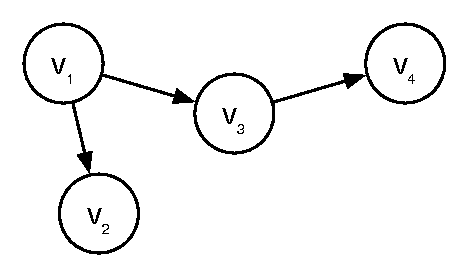
\includegraphics[scale=0.8]{simple-graph-example.pdf}
\caption{A simple graph.}
\label{fig: simple-example}
\end{figure}

Graphs are a natural way of expressing many problems in mathematics and computer science. They are also useful for representing programs internally in a compiler. One of the seminal graph representations is the Control Flow Graph (CFG), which was introduced by Allen \cite{808479} to explicitly represent possible control paths in a program. In the CFG, vertices are called basic blocks and contain straight-line instructions. When control enters a basic block, all instructions must be executed in that block. The edges that connect basic blocks together represent transfer of the control flow. An illustration of a CFG can be seen in Figure~\ref{fig: example-cfg}, showing a translation between some three-address code and the resulting graph. The CFG is used to convert a program into SSA form \cite{115320}. Additionally, representing a program in this way makes a number of operations simpler to perform, such as identifying loops, discovering irreducibility and performing interval analysis techniques.

\begin{figure}[ht]
\centering
\subfigure{
	\begin{minipage}[b]{0.3\linewidth}
	\texttt{\begin{tabbing}
	1: \=a = 0; \\
	\> b = 0; \\
	2: \> if x $>=$ y goto 4 \\
	3: \> a = x; \\
	\> goto 5; \\
	4: \> a = y; \\
	5: \> if a $>=$ y goto 6 \\
	\> a = a * x;\\
	\> a = a + b;\\
	\> b = b + 1;\\
	\> goto 5; \\
	6: \> ret a + b; \\
	\end{tabbing}}
	\end{minipage}
}
\subfigure{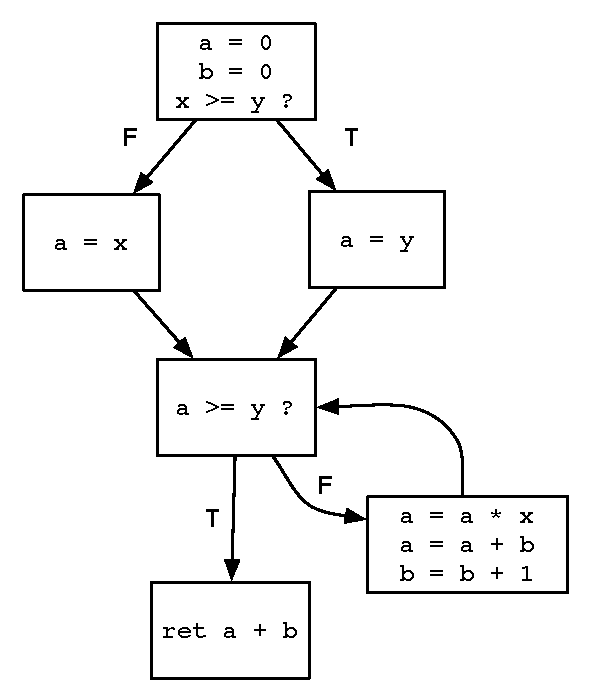
\includegraphics[scale=0.55]{cfg-example.pdf}}
\caption{Some three address code and the resulting CFG after translation.}
\label{fig: example-cfg}
\end{figure}

The CFG models control flow, but many graphs model \textit{data flow}. The graphs we consider in this section are all data flow graphs, representing the data dependences in a program. We will look at a number of different SSA-based graph representations. These range from those which are a very literal translation of SSA into a graph format to those which are more abstract in nature. An introduction to each graph will be given, along with diagrams to show how sample programs look when translated into that particular graph. Additionally, we will touch on the literature describing the usage of a graph and see why it was useful for that particular application.

\section{The SSA Graph}

We begin our exploration with a graph that is very similar to SSA. Many different definitions exist in the literature, so we take ours from Cooper et al \cite{504710}. An SSA Graph consists of vertices which represent operations (such as \texttt{add} and \texttt{load}) or $\mathtt{\phi}$-functions, and edges connect uses to definitions. For example, the incoming edges to a vertex represent the arguments required for that operation, and the outgoing edge from a vertex represents the propagation of that operation's result after it has been computed. This graph is therefore a \textit{demand-based} representation. In order to compute a vertex, we must \textit{demand} the results of the operands and then perform the operation indicated on that vertex. The SSA Graph can be constructed from a program in SSA form by adding use-definition chains. We present some sample code in Figure~\ref{fig: ssa-graph-example-code}. This is translated into an SSA Graph in Figure~\ref{fig: ssa-graph-example-graph}. Note that there are no explicit nodes for variables in the graph. Instead, an operator node can be seen as the ``location'' of the value stored in a variable. We have annotated operators with variable names to show the correspondence between the operations in the graph and in the SSA form program.

% TODO: proper centering of this code? Looks a bit crap at the moment.
\begin{figure}[ht]
\centering
\subfigure{
	\begin{minipage}[b]{0.3\linewidth}
	\texttt{\begin{tabbing}
	begin: \= a = 0; \\
	\> i = 0; \\
	loop: \> a = a * i; \\
	\> i++; \\
	\> if i < 100 goto loop;\\
	end: \> print(a + i);
	\end{tabbing}}
	\end{minipage}
}
\subfigure{
	\begin{minipage}[b]{0.3\linewidth}
	\texttt{\begin{tabbing}
	begin: \=$a_{0}$ = 0; \\
	\> $i_{0}$ = 0; \\
	loop: \> $a_{1}$ = $\phi$($a_{0}$,$a_{2}$); \\
	\> $i_{1}$ = $\phi$($i_{0}$,$i_{2}$); \\
	\> $a_{2}$ = $a_{1}$ * $i_{1}$; \\
	\> $i_{2}$ = $i_{1}$ + 1; \\
	\> if $i_{2}$ < 100 goto loop;\\
	end: \> $a_{3}$ = $\phi$($a_{1}$,$a_{2}$); \\
	\> $i_{3}$ = $\phi$($i_{1}$,$i_{2}$); \\
	\> print($a_{3}$ + $i_{3}$);
	\end{tabbing}}
	\end{minipage}
}
\caption{Some sample code translated into SSA form.}
\label{fig: ssa-graph-example-code}
\end{figure}

The key benefit of representing the input program in this form is that the compiler writer is able to apply a wide array of graph-based optimizations by using standard graph traversal and transformation techniques. This can make many optimizations much easier to perform than on the standard linear SSA form, especially when the focus is on loop optimization. Some work \cite{1375663} with the SSA Graph also models memory dependencies. This is achieved by augmenting the graph with additional edges that enforce an order of interpretation. These edges are extensively used in the Value State Dependence Graph, which we will look at next.

In the literature, the SSA Graph has been used to detect a variety of induction variables in loops \cite{143131,201003}, also for performing instruction selection techniques \cite{1375663,1269857}, operator strength reduction \cite{504710}, rematerialization \cite{143143}, and has been combined with an extended SSA language to aid compilation in a parallelizing compiler \cite{Stoltz_extendedssa}. The reader should note that the exact specification of what constitutes an SSA Graph changes from paper to paper. The essence of the IR is presented here, as each author tends to make small modifications for their particular implementation.

\begin{figure}
\centering
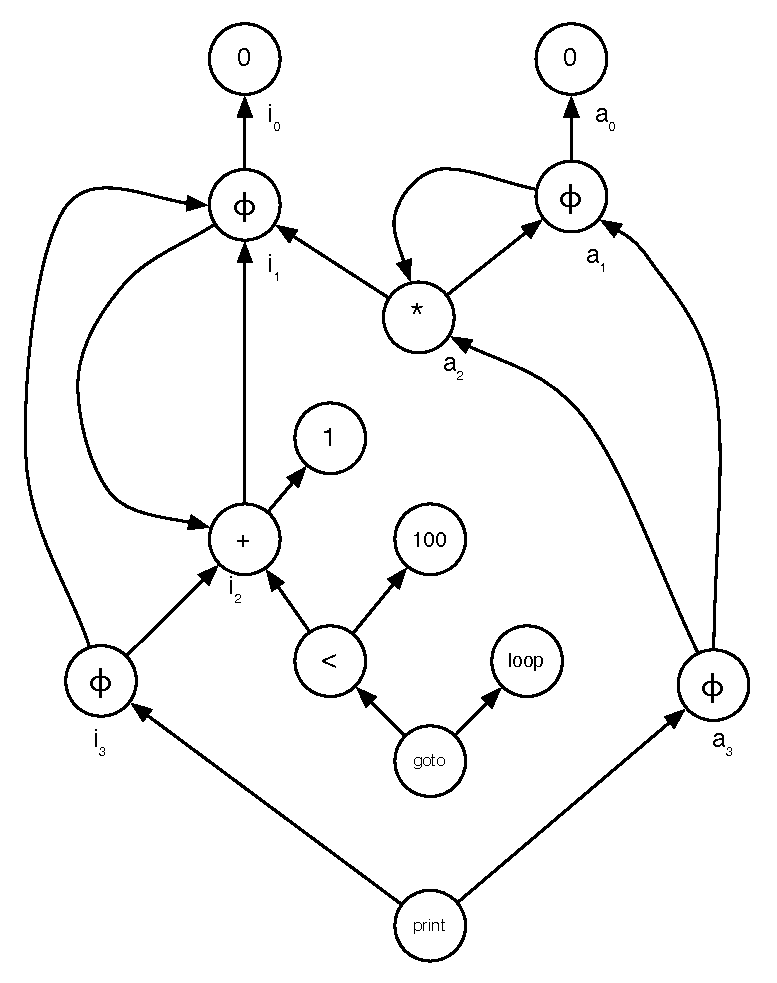
\includegraphics[scale=0.5]{ssa-graph.pdf}
\label{fig: ssa-graph-example-graph}
\caption{Our sample program translated into an SSA Graph.}
\end{figure}

\section{Gating functions}

In SSA form, $\phi$-functions are used to identify points where variable definitions converge. However, they cannot be directly interpreted, as they do not specify the condition which states which of the variable definitions to choose. By this logic, we cannot directly interpret the SSA Graph. Being able to interpret our IR is a useful property as it gives the compiler writer more information when implementing optimizations, and also reduces the complexity of performing code generation. Gated Single Assignment form  is an extension of SSA with \textit{gating functions}. These gating functions are directly interpretable versions of $\phi$-nodes, and replace $\phi$-nodes in the representation. There are three forms of gating function:

\begin{itemize}
\item The $\gamma$ function explicitly represents the condition which determines which $\phi$ value to select. A $\gamma$ function is of the form $\gamma(P,V_{1},V_{2})$ where $P$ is a predicate, and $V_{1}$ and $V_{2}$ are the values to be selected if the predicate evaluates to true or false respectively. This can be read simply as \textit{if-then-else}. 
\item The $\mu$ function is inserted at loop headers to select the initial and loop carried values. A $\mu$ function is of the form $\mu(V_{init},V_{iter})$, where $V_{init}$ is the initial input value for the loop, and $V_{iter}$ is the iterative input. We replace $\phi$-functions at loop headers with $\mu$ functions.
\item The $\eta$ function determines the value of a variable when a loop terminates. An $\eta$ function is of the form $\eta(P,V_{final})$ where $P$ is a predicate and $V_{final}$ is the definition reaching beyond the loop.
\end{itemize}

These gating functions are important as the concept will form components of other IRs in this chapter. GSA has seen a number of uses in the literature. The first was by Ballance et al. \cite{93578} as a component of the Program Dependence Web IR. Havlak \cite{Havlak93constructionof} presents an algorithm for construction of a simpler version of GSA -- Thinned GSA -- which is constructed from a CFG in SSA form. Tu and Padua \cite{207115} present an algorithm that constructs SSA and GSA simultaneously in a single process. We leave further investigation of the construction algorithms as an exercise to the reader as they are lengthly and beyond the scope of this chapter. 

It is easiest to understand these gating functions by means of an example. Figure~\ref{fig: gsa-graph-example} shows how our earlier code example in Figure~\ref{fig: ssa-graph-example-code} translates into GSA form. Here, we can see the use of both $\mu$ and $\eta$ gating functions. At the header of our sample loop the $\phi$-functions have been replaced by $\mu$ functions which determines between the initial and iterative values of \texttt{a} and \texttt{i}. After the loop has finished executing, the two $\eta$ functions which propagate the correct value from the corresponding $\mu$ function.

% TODO: label is wrong when compiled?
\begin{figure}
\centering
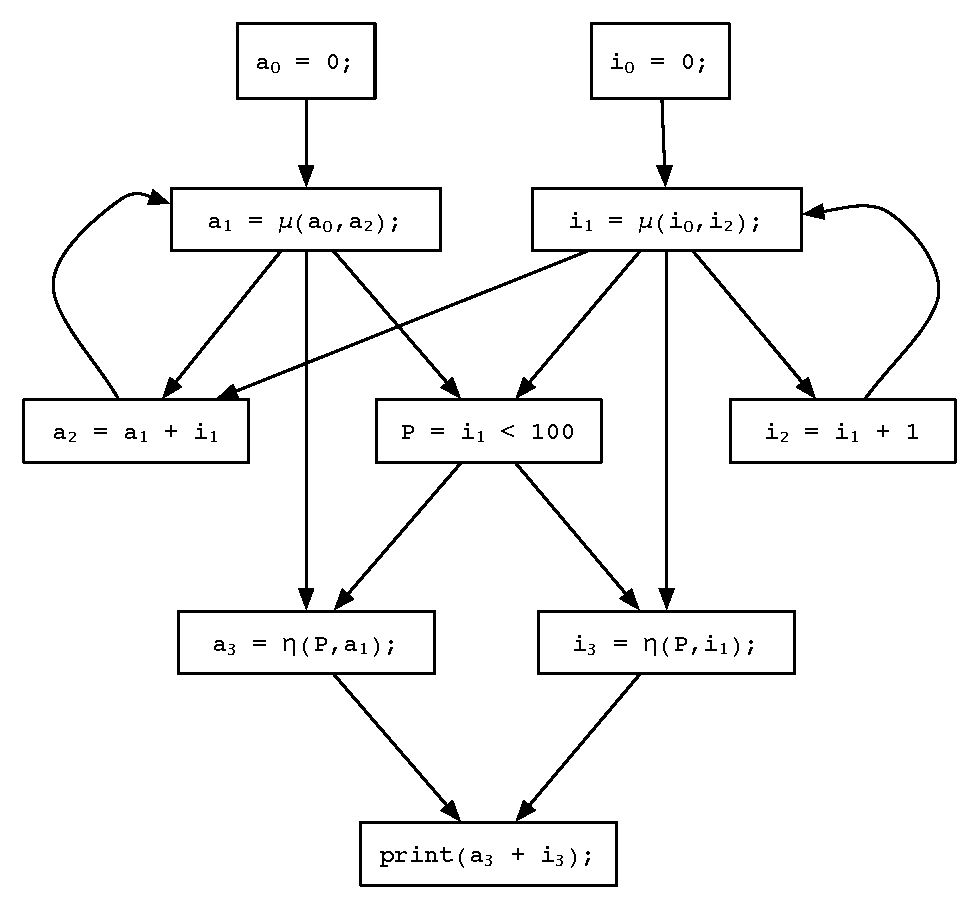
\includegraphics[scale=0.55]{gsa-example.pdf}
\label{fig: gsa-graph-example}
\caption{A graph representation of our sample code in GSA form.}
\end{figure}

% TODO: end of GSA section
%By using gating functions it becomes possible to construct IRs based solely on data dependencies that are sparse in nature. We will look at one of these in the next section.

% TODO: VSDG
\section{Towards the Value State Dependence Graph}

The gating functions defined in the previous section were used in the development of a sparse data-flow graph intermediate representation called the Value Dependence Graph (VDG) \cite{177907}. The VDG represents programs as value (data) dependencies and does not contain any control flow information. In the VDG, there is an edge $(n,v)$, drawn as an arrow $n\rightarrow v$, if a node $n$ requires the value $v$ in order to compute its own value. The key benefit of this representation is that there is no enforced ordering of operations. 

Selection in the VDG is represented by $\gamma$-nodes, which implement the same behavior as the $\gamma$ gating function. Function calls and loops are represented by $\lambda$-nodes, with loop bodies translated into tail recursive functions. However, there was a problem with the VDG: failure to preserve the terminating properties of a program. The original paper states that \textit{``Evaluation of the VDG may terminate even if the original program would not...''}. This problem was addressed in the creation of the Value State Dependence Graph (VSDG) \cite{UCAM-CL-TR-607}. We take our definition from Johnson and Mycroft. \cite{Johnson_combinedcode}

The VSDG is a directed graph consisting of operation nodes, loop and merge nodes together with value- and state-dependency edges. A VSDG represents a single procedure in a program. A formal definition of the VSDG is as follows:

\begin{definition}
A VSDG is a labelled direct graph $G=(N,E_{V},E_{S},\ell,N_{0},N_{\infty})$ consisting of nodes $N$ (with unique entry node $N_{0}$ and exit node $N_{\infty}$), value-dependency edges $E_{V}\subseteq N\times N$, state-dependency edges $E_{S}\subseteq N \times N$. The labelling function $\ell$ associates each node with an operator.
\end{definition}

Value dependencies ($E_{V}$) indicate the flow of values between nodes, and this must be preserved during optimization and transformations. State dependencies ($E_{S}$) represent  the essential sequential dependency required by the input program, e.g. a particular load instruction must follow a store instruction without being reordered. An edge $(n_{1},n_{2})$ represents the flow of data or control \textit{from} $n_{1}$ to $n_{2}$. To get a basic visual picture of the graph, we show a recursive factorial function written in pseudocode in Figure ~\ref{fig: vsdg-fac} which is then translated into a VSDG. This demonstrates the key components of the graph. Value dependency edges are drawn as solid lines, and state dependency edges as dashed ones. We see a \texttt{call} node for the function call, a \texttt{const} node for the function label and the integer 1, an equality node, two $\gamma$-nodes and function entry and exit nodes. We tend to refer to nodes having labelled \textit{ports} to describe interaction with them.

\begin{figure}[ht]
\centering
\subfigure{
	\begin{minipage}[b]{0.3\linewidth}
	\texttt{\begin{tabbing}
	code here
	\end{tabbing}}
	\end{minipage}
}
\subfigure{
\includegraphics[scale=0.55]{vsdg-fac.pdf}}
\caption{Some pseudocode for a recursive factorial function which is then translated into an equivalent VSDG.}
\label{fig: vsdg-fac}
\end{figure}

There are two well-formedness conditions for the VSDG that must be satisfied. $\ell$ and the arity of $E_{V}$ must be consistent, e.g. an addition operator must have two inputs. The VSDG must also correspond to a structured program, e.g. there are no loops in the VSDG that are not mediated by loop nodes. A VSDG is implicitly in SSA form, which is a property inherited from the VDG. For any given operator node $n$, $n$ will have zero or more $E_{V}$-successors using its value. We will now describe the different components constituting the VSDG.

\subsection{Nodes}

We use four main classes of VSDG nodes. These are value nodes (pure arithmetic), $\gamma$-nodes (conditional statements), $\theta$-nodes (loop constructs) and state nodes (side-effecting operations).

\begin{description}
\item[Value nodes] Most VSDG nodes generate a value form a computation, e.g. an addition or subtraction, which is applied to the values that they depend upon.
\item[$\gamma$-nodes] The $\gamma$-node functions similarly to the $\gamma$ gating function. We define it as follows:
\begin{definition}
A $\gamma$-node $\gamma(C,T,F)$ evaluates the condition dependency $C$, and returns the value of $T$ if $C$ is true, otherwise $F$.
\end{definition}
\item[$\theta$-nodes] The $\theta$-node models the iterative behaviour of loops. It uses the notion of an internal value which may be updated on each subsequent iteration. It has five different ports, defined as follows:
\begin{definition}
A $\theta$-node $\theta(C,I,R,L,X)$ sets its internal value to initial value $I$ then, while condition value $C$ holds true, sets $L$ to the current internal value and updates the internal value with the repeat value $R$. When $C$ evaluates to false computation ceases and the last internal value is returned through the $X$ port.
\end{definition}
As an example, a loop which updates $k$ variables with have the following: a single condition port $C$, initial-value ports $I_{1},...,I_{k}$, loop iteration ports $L_{1},...,L_{k}$, loop return ports $R_{1},...,R_{k}$, and loop exit ports $X_{1},...,X_{k}$. The $\theta$-node directly implements pre-test loops (\texttt{while}, \texttt{for}), with post-test loops (\texttt{do...while}, \texttt{repeat...until}) synthesised from a pre-test loop preceded by a duplicate of the loop body. %TODO: example figure
\end{description}

\subsection{State nodes}



% Key components
% Usage/implementation/optimizations using it
% Further work

\newpage
% =================
% Abstract is below here.
% =================

\section*{Abstract}

\subsection*{Introduction}

This chapter will explore some approaches to using SSA concepts in graph-based intermediate representations. I'm leaving the abstract here for the time being, although it seems to be changing as I write.

\subsection*{SSA Graph}

A literal translation of SSA into a graph. Introduction, examples and uses in the literature are shown.

\subsection*{The gating function}

One problem with SSA is the difficulty of directly interpreting $\phi$-functions as there is no way to explicitly tell at compile-time which of the $\phi$-variables will be chosen. This introduces the idea of the gating function -- called the $\gamma$-node -- which was introduced by Tu and Padua \cite{207115} and used by Ballance et al. in the Program Dependence Web\cite{93578} representation. We give some examples for explanation of $\phi$-translation, showing how it translates $\phi$-functions into $\gamma$-functions.
We give some construction examples and show how loops are handled with $\mu$ and $\eta$ style representations.

\subsection*{Value State Dependence Graph}

The Value State Dependence Graph (VSDG) is an intermediate representation for modeling programs using data dependencies. It can be seen as a spiritual successor to the Value Dependence Graph\cite{177907}, with the addition of ``state" edges to allow only the essential sequential dependences in a program to constrain the ordering of instructions. The IR was introduced by Johnson\cite{UCAM-CL-TR-607}, with further developments by Upton\cite{upton} and Lawrence\cite{UCAM-CL-TR-705}.

We give an outline of the key features of the VSDG and show how it is implicitly in SSA form. Construction is discussed with reference to Johnson's work. We then explain how the representation lends itself well to optimizations due to the adaptable nature of the graph. Discussion then focuses on the difficulties of generating sequential code from the graph\cite{DBLP:conf/pdpta/Upton03}, and Lawrence's proposed compiler architecture. We conclude with possible directions for ongoing work with the VSDG.

\subsection*{VSDG application: Combined Code Motion and Register Allocation}

Johnson and Mycroft \cite{johnson-combined} present an algorithm which performs code motion and register allocation at the same time by using the VSDG, uniting two phases which were traditionally believed to be antagonistic. We explore this algorithm and show how it works.


